% =============================================================
% Codebook 主檔說明
% - 目標：在最少頁數內排入常用演算法 / 資料結構程式碼。
% - 版面：使用 twocolumn 壓縮，手動設定窄邊界，字體縮小。
% - 編譯：建議使用 xelatex (需支援 fontspec / xeCJK)。
% - 可調整項目：行號 (listings)、字型、是否加入更多章節。
% =============================================================
\documentclass[a4paper,10pt,twocolumn,oneside]{article}
\setlength{\columnsep}{10pt}                                                              %兩欄模式的間距
\setlength{\columnseprule}{0pt}                                                                %兩欄模式間格線粗細

\usepackage{amsthm}								%定義，例題
\usepackage{amssymb}
%\usepackage[margin=2cm]{geometry}
\usepackage{fontspec}								%設定字體
\usepackage{color}
\usepackage[x11names]{xcolor}
\usepackage{listings}								%顯示code用的
%\usepackage[Glenn]{fncychap}						%排版，頁面模板
\usepackage{fancyhdr}								%設定頁首頁尾
\usepackage{graphicx}								%Graphic
\usepackage{enumerate}
\usepackage{titlesec}
\usepackage{amsmath}
\usepackage{tikz}
\usepackage{xpatch}
\usepackage[CheckSingle, CJKmath]{xeCJK}
% \usepackage{CJKulem}
%\usepackage[T1]{fontenc}
\titlespacing{\section}{0cm}{0cm}{0cm}
\titlespacing{\subsection}{0cm}{0cm}{0cm}
\usepackage{amsmath, courier, listings, fancyhdr, graphicx}
\topmargin=0pt
\headsep=5pt
\textheight=780pt
\footskip=0pt
\voffset=-40pt
\textwidth=545pt
\marginparsep=0pt
\marginparwidth=0pt
\marginparpush=0pt
\oddsidemargin=0pt
\evensidemargin=0pt
\hoffset=-42pt

%\renewcommand\listfigurename{圖目錄}
%\renewcommand\listtablename{表目錄} 

%%%%%%%%%%%%%%%%%%%%%%%%%%%%%


\setmainfont [				%主要字型
Path = .fonts/ttf/,
UprightFont = *-Regular,
BoldFont = *-Bold,
ItalicFont = *-Italic
] {Consolas}

\setmonofont [        
    Path = .fonts/ttf/,
    UprightFont = *-Regular
    ] {Monaco}
    
    \setCJKmainfont[
        Path = .fonts/ttf/,        % 你放字型檔的資料夾（相對於主 .tex 檔案）
        Extension = .ttf,
        UprightFont = *-Regular,
        BoldFont = *-Bold,
        ]{NotoSansTC}
        
        \XeTeXlinebreaklocale "zh"						%中文自動換行
        \XeTeXlinebreakskip = 0pt plus 1pt				%設定段落之間的距離
        \setcounter{secnumdepth}{3}						%目錄顯示第三層
        
        %%%%%%%%%%%%%%%%%%%%%%%%%%%%%
        \makeatletter
        \lst@CCPutMacro\lst@ProcessOther {"2D}{\lst@ttfamily{-{}}{-{}}}
        \@empty\z@\@empty
        \makeatother
        \lstset{											% Code顯示
        language=C++,										% the language of the code
        basicstyle=\footnotesize\ttfamily, 						% the size of the fonts that are used for the code
        %numbers=left,										% where to put the line-numbers
        numberstyle=\footnotesize,						% the size of the fonts that are used for the line-numbers
        stepnumber=1,										% the step between two line-numbers. If it's 1, each line  will be numbered
        numbersep=5pt,										% how far the line-numbers are from the code
        backgroundcolor=\color{white},					% choose the background color. You must add \usepackage{color}
        showspaces=false,									% show spaces adding particular underscores
        showstringspaces=false,							% underline spaces within strings
        showtabs=false,									% show tabs within strings adding particular underscores
        frame=false,											% adds a frame around the code
        tabsize=2,											% sets default tabsize to 2 spaces
        captionpos=b,										% sets the caption-position to bottom
        breaklines=true,									% sets automatic line breaking
        breakatwhitespace=false,							% sets if automatic breaks should only happen at whitespace
        escapeinside={\%*}{*)},							% if you want to add a comment within your code
        morekeywords={*},									% if you want to add more keywords to the set
        keywordstyle=\bfseries\color{Blue1},
        commentstyle=\itshape\color{Red4},
        stringstyle=\itshape\color{Green4},
        }
        
        %%%%%%%%%%%%%%%%%%%%%%%%%%%%%
        
        % \usepackage{verbatim}
        \begin{document}
        \pagestyle{fancy}
        \fancyfoot{}
        %\fancyfoot[R]{\includegraphics[width=20pt]{ironwood.jpg}}
        \fancyhead[L]{NTOU AsdHater}
        \fancyhead[R]{\thepage}
        \renewcommand{\headrulewidth}{0.4pt}
        \renewcommand{\contentsname}{Contents} 
        
        \newcommand{\includetex}[2]{
            \subsection{#1}
            \input{#2}
            \vspace{-1.2em}
            }
            \scriptsize
            \tableofcontents
            
            % \newpage
            %sectionstart  % ===== 以下依分類匯入各程式碼檔案 =====
\section{Basic}
    \subsection{Default}
    \lstinputlisting{Basic/Default.cpp}

    \subsection{builtin}
    \lstinputlisting{Basic/builtin.cpp}

    \subsection{random}
    \lstinputlisting{Basic/random.cpp}

    \subsection{run.bat}
    \lstinputlisting{Basic/run.bat}

    \subsection{run.sh}
    \lstinputlisting{Basic/run.sh}

\section{Data Structure}
    \subsection{Segment Tree}
    \lstinputlisting{DataStructure/segtree.cpp}

    \subsection{segment Tree2}
    \lstinputlisting{DataStructure/segtree2.cpp}

    \subsection{BIT}
    \lstinputlisting{DataStructure/BIT.cpp}

    \subsection{離散化}
    \lstinputlisting{DataStructure/離散化.cpp}

    \subsection{DSU}
    \lstinputlisting{DataStructure/DSU.cpp}

    \subsection{Kruskal}
    \lstinputlisting{DataStructure/Kruskal.cpp}

\section{Graph}
    \subsection{BCC}
    \lstinputlisting{Graph/BCC.cpp}

    \subsection{SCC}
    \lstinputlisting{Graph/SCC.cpp}

    \subsection{支配樹}
    \lstinputlisting{Graph/DominatorTree.cpp}

    \subsection{最大團}
    \lstinputlisting{Graph/MaxClique.cpp}

    \subsection{Topo}
    \lstinputlisting{Graph/topo.cpp}

    \subsection{找環}
    \lstinputlisting{Graph/FindCircle.cpp}

    \subsection{無向圖環路徑}
    \lstinputlisting{Graph/NFindCirclePath.cpp}

    \subsection{有向圖環路徑}
    \lstinputlisting{Graph/FindCirclePath.cpp}

    \subsection{無向圖歐拉路徑}
    \lstinputlisting{Graph/NEulerPath.cpp}

    \subsection{SPFA}
    \lstinputlisting{Graph/spfa.cpp}

    \subsection{01bfs}
    \lstinputlisting{Graph/01bfs.cpp}

    \subsection{dijk}
    \lstinputlisting{Graph/dijk.cpp}

    \subsection{flow/dinic}
    \lstinputlisting{Graph/dinic_BCW.cpp}

    \subsection{flow/ISFP}
    \lstinputlisting{Graph/ISFP.cpp}

    \includetex{結論}{Graph/Conclusion.tex} % 圖論補充 / 結論整理

\section{geometry}
    \subsection{Point}
    \lstinputlisting{geometry/Point.cpp}

    \subsection{Line}
    \lstinputlisting{geometry/Line.cpp}

    \subsection{Circle}
    \lstinputlisting{geometry/Circle.cpp}

    \subsection{點線距離}
    \lstinputlisting{geometry/PointToSegmentDistance.cpp}

    \subsection{線段相交}
    \lstinputlisting{geometry/線段相交.cpp}

    \subsection{inPolygon}
    \lstinputlisting{geometry/inpoly.cpp}
    
    \subsection{ConvexHull}
    \lstinputlisting{geometry/ConvexHull.cpp}
    
    \subsection{最小圓覆蓋}
    \lstinputlisting{geometry/最小圓覆蓋.cpp}
    
    \subsection{旋轉卡尺}
    \lstinputlisting{geometry/旋轉卡尺.cpp}
    

\section{Tree}

    \subsection{is\_anc}
    \lstinputlisting{Tree/isanc.cpp}

    \subsection{LCA}
    \lstinputlisting{Tree/LCA.cpp}

    \subsection{倍增}
    \lstinputlisting{Tree/倍增.cpp}

    \subsection{tree\_flaten}
    \lstinputlisting{Tree/tree\_flaten.cpp}


\section{DP}
    \subsection{LIS}
    \lstinputlisting{DP/LIS.cpp}

    \subsection{LCS}
    \lstinputlisting{DP/LCS.cpp}

    \subsection{拆分}
    \lstinputlisting{DP/二進制拆分.cpp}

    \subsection{編輯距離}
    \lstinputlisting{DP/編輯距離.cpp}

    \subsection{SOSDP}
    \lstinputlisting{DP/SOSDP.cpp}

    \subsection{p\_median}
    \lstinputlisting{DP/pmedian.cpp}

\section{search}
    \subsection{binary search}
    \lstinputlisting{Search/binary.cpp}
    
    \subsection{三分搜}
    \lstinputlisting{Search/三分搜.cpp}

\section{Math}
    \subsection{質數篩}
    \lstinputlisting{Math/sieve.cpp}

    \subsection{fpow}
    \lstinputlisting{Math/fpow.cpp}

    \subsection{exgcd}
    \lstinputlisting{Math/exgcd.cpp}

    \subsection{組合數}
    \lstinputlisting{Math/組合數.cpp}

    \subsection{josephus}
    \lstinputlisting{Math/josephus.cpp}

    \subsection{josephus2}
    \lstinputlisting{Math/josephus2.cpp}

    \subsection{FFT}
    \lstinputlisting{Math/FFT.cpp}

    \subsection{Matrices\_fpow}
    \lstinputlisting{Math/Matrices_fpow.cpp}

    \subsection{Miller-Rabin}
    \lstinputlisting{Math/Millar\_Rabin.cpp}

    \subsection{pollard rho}
    \lstinputlisting{Math/pollard\_rho.cpp}



\section{String}
    \subsection{KMP}
    \lstinputlisting{String/KMP.cpp}

    \subsection{AC自動機}
    \lstinputlisting{String/AC自動機.cpp}
    
    \subsection{minRotation}
    \lstinputlisting{String/minRotation.cpp}

    \subsection{迴文樹}
    \lstinputlisting{String/PalTree.cpp}

    \subsection{Rolling Hash}
    \lstinputlisting{String/RollingHash.cpp}

    \subsection{SAIS}
    \lstinputlisting{String/SAIS.cpp}

    \subsection{trie}
    \lstinputlisting{String/trie.cpp}

    \subsection{z\_value}
    \lstinputlisting{String/z\_value.cpp}

    \subsection{馬拉車}
    \lstinputlisting{String/馬拉車.cpp}
    
%sectionend  % ===== 程式碼主體結束 =====
    \section{好東西}
        \includetex{大悲咒}{大悲咒} % 附錄 / 其他補充
        \vspace*{1cm}
        \includetex{心經}{心經中日文} % 附錄 / 其他補充
    \clearpage % 強制換到新的一頁

% 使用 listings 匯入，設定基本的等寬字型，不顯示行號，不套用 C++ 高亮
\lstinputlisting[
    language={},         % 純文字，不使用程式語言高亮
    numbers=none,        % 不顯示行號（否則 ASCII 畫會被行號破壞）
    basicstyle=\ttfamily % 確保使用等寬字型，畫面才不會歪掉
]{濕婆} 


% 方格紙 (下方巨集)：列印時可附加數頁空白格紙供賽中手寫推導。
% 若不需要可註解整段，或改為插入外部 PDF 模板以加速編譯。
% 方格紙
\newcommand{\halfgridpage}{
    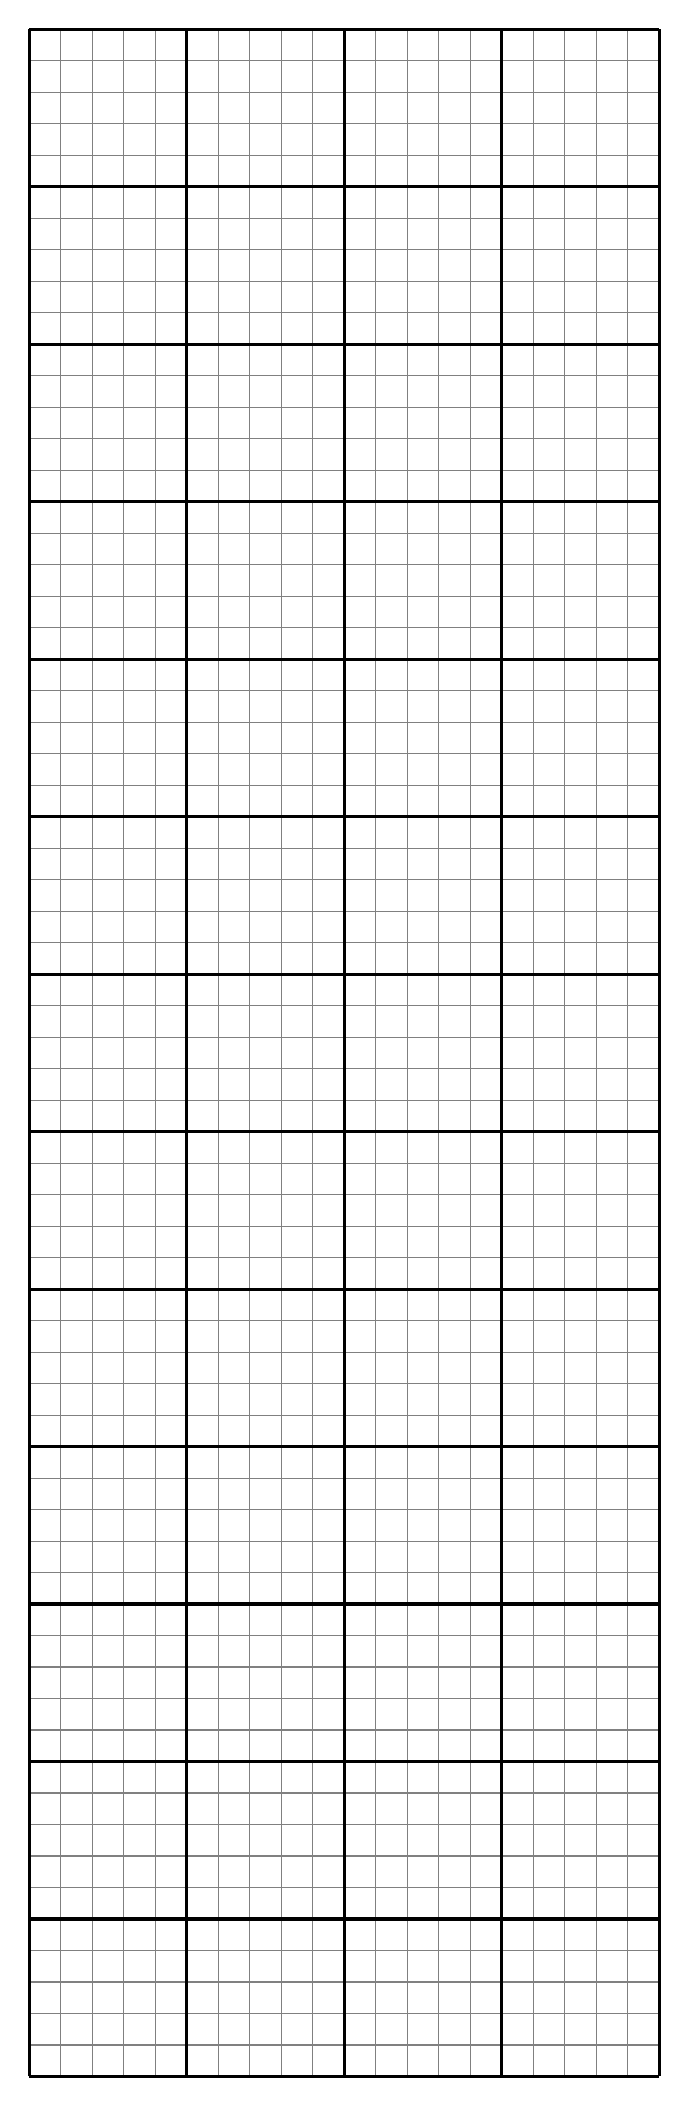
\begin{tikzpicture}[every node/.style={minimum size=1cm-\pgflinewidth, outer sep=10pt}, scale=2]
        \draw[step=0.2cm,color=gray] (0,0) grid (4,13);
        \draw[step=1cm,color=black,line width=0.4mm] (0,0) grid (4,13);
    \end{tikzpicture}
    \newpage
}
\newcommand{\gridpage}{
    \centering
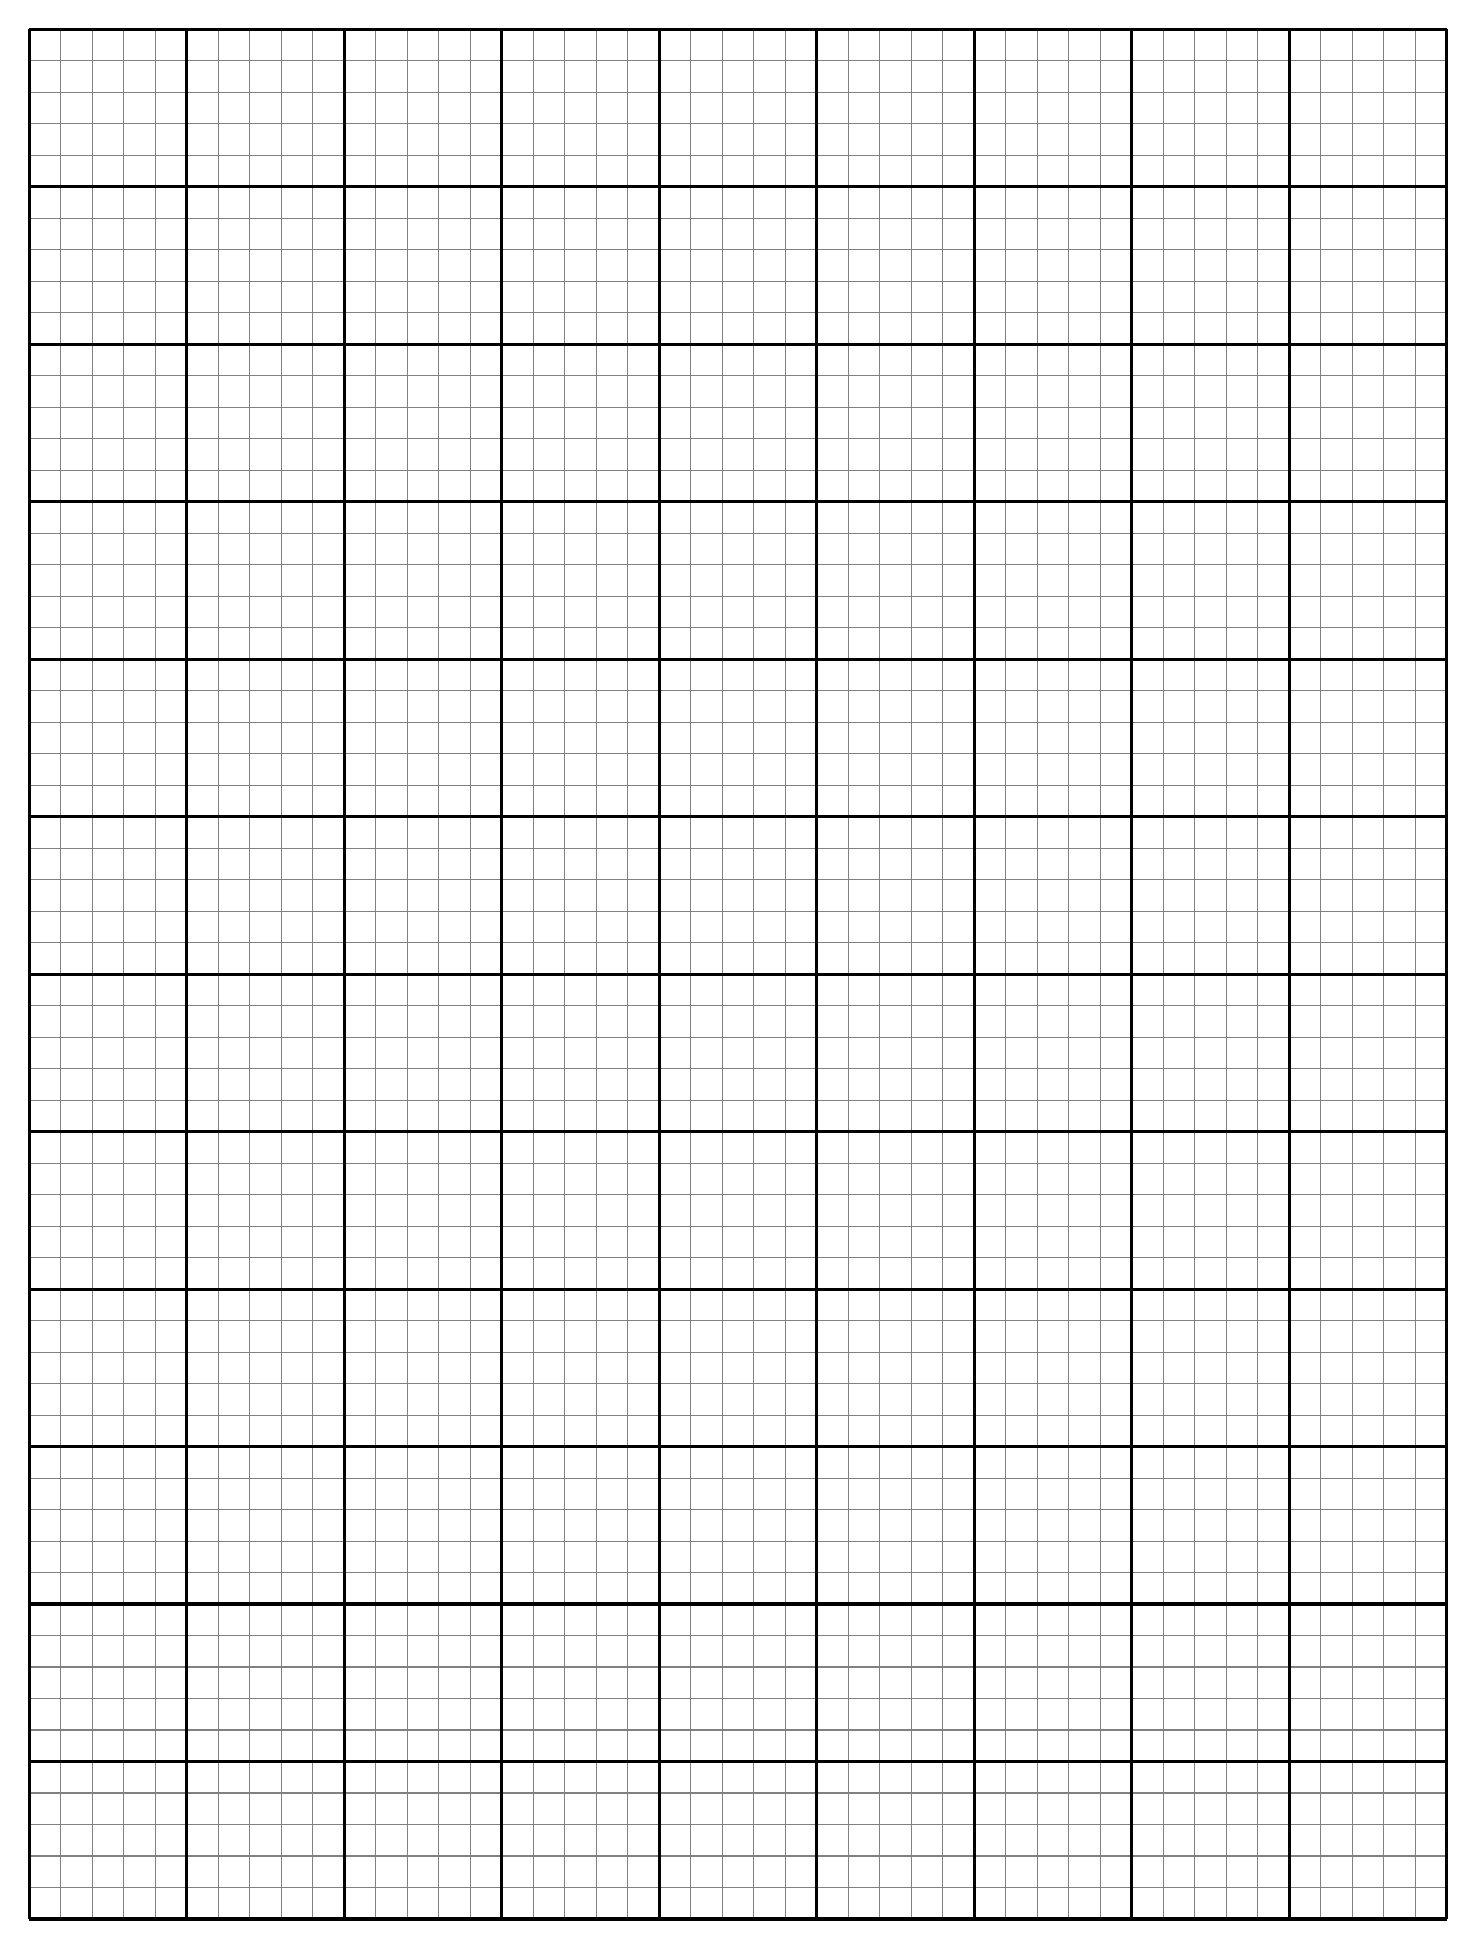
\begin{tikzpicture}[every node/.style={minimum size=1cm-\pgflinewidth, outer sep=10pt}, scale=2]
    \draw[step=0.2cm,color=gray] (0,0) grid (9,12);
    \draw[step=1cm,color=black,line width=0.4mm] (0,0) grid (9,12);
\end{tikzpicture}
    \newpage
}
\onecolumn
\gridpage
\gridpage
% \gridpage
% \gridpage
% \gridpage


\end{document}
